\documentclass[tikz]{standalone}

\usetikzlibrary{patterns}

\def\radius{1}

\begin{document}
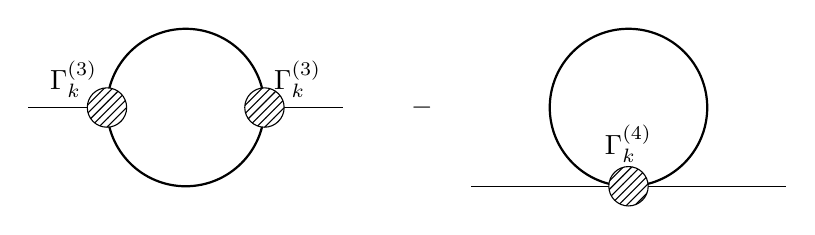
\begin{tikzpicture}

  % Left diagram
  \draw[thick] (0,0) circle (\radius);
  \draw (-2*\radius,0) -- (-\radius,0) (\radius,0) -- (2*\radius,0);

  \draw[fill=white,postaction={pattern=north east lines}] (\radius,0) circle (0.25*\radius) node[above right] {$\Gamma_k^{(3)}$} (-\radius,0) circle (0.25*\radius) node[above left] {$\Gamma_k^{(3)}$};

  \node at (3*\radius,0) {$-$};

  % Right diagram
  \begin{scope}[xshift=160]
    \draw[thick] (0,0) circle (\radius);
    \draw (-2*\radius,-\radius) -- (2*\radius,-\radius);

    \draw[fill=white,postaction={pattern=north east lines}] (0,-\radius) circle (0.25*\radius) node[above=5pt] {$\Gamma_k^{(4)}$};
  \end{scope}

\end{tikzpicture}
\end{document}
